\chapter{Ausarbeitung}
\section{Aufgabe 1}
Die Drehraten sind von der Erdrotation befreit: $\omega_e = 0$, das gilt:
\begin{equation*}
	\bm{\omega}_{ep}^p = \bm{\omega}_{ip}^p
\end{equation*}
$\bm{\omega}_{ip}^p$ sind die gemessene Drehraten, die Elementen von $\bm{A}$ Matrix sind bekannt. 
\begin{gather*}
	\bm{q}(t+\Delta t) = e^{\frac{\bm{A} \Delta t}{2}} \cdot \bm{q}(t) \\
	\bm{q}(0) = \begin{bmatrix}
		1 \\
		0 \\
		0 \\
		0
	\end{bmatrix}
\end{gather*}
Für jede Epoche sind dann DCM mit $\bm{q}$ bestimmbar, dann gibt es:
\begin{gather*}
	\bm{g}^{e} = -9,81 \cdot \frac{\bm{x}}{|\bm{x}|} \\
	\dot{\bm{v}}^{e} = \bm{C} \bm{a}^{p} + \bm{g}^{e} \\
	\bm{v}^{e}(t) = \bm{v}^{e}(t-1) + \dot{\bm{v}}^{e} \cdot \Delta t \\
	\bm{x}^{e}(t) = \bm{x}^{e}(t-1) + \bm{v}^{e} \cdot \Delta t
\end{gather*}
Die Trajektorie liegt in \autoref{fig:Trajektorie}. Sie liegt in x-z Ebene und wölbt sich nach innen. 
\begin{figure}[htbp]
	\centering
	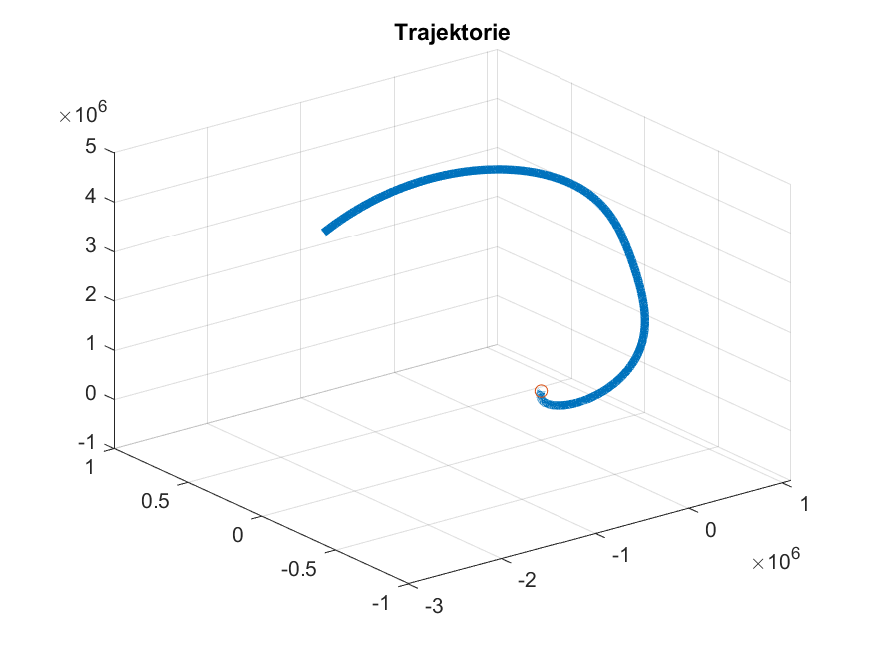
\includegraphics[width=0.9\textwidth]{images/Trajektorie} 
	\caption{Trajektorie} 
	\label{fig:Trajektorie}
\end{figure}\\\\
$\sqrt{x^2 + y^2 + z^2}$ sind immer kleiner als Erdradius, deswegen ist der Verlauf nicht realistisch.
\clearpage
\section{Aufgabe 2}

















